
\documentclass[twoside]{article}
\setlength{\oddsidemargin}{0.25 in}
\setlength{\evensidemargin}{-0.25 in}
\setlength{\topmargin}{-0.6 in}
\setlength{\textwidth}{6.5 in}
\setlength{\textheight}{8.5 in}
\setlength{\headsep}{0.75 in}
\setlength{\parindent}{0 in}
\setlength{\parskip}{0.1 in}


\usepackage{amsmath,amsfonts,graphicx,amssymb}
\usepackage{graphicx}
\usepackage{float}
\usepackage{hyperref}
\hypersetup{
    colorlinks=true,
    linkcolor=blue,
    filecolor=magenta,      
    urlcolor=cyan,
}
\usepackage{titlesec}
\usepackage{subfigure}
\usepackage{xcolor}
\usepackage{color, soul}
\graphicspath{ {./} }
\titlespacing*{\section}
{0pt}{5.5ex plus 1ex minus .2ex}{4.3ex plus .2ex}


\newcommand{\lecture}[2]{
   \pagestyle{myheadings}
   \thispagestyle{plain}
   \newpage
%    \setcounter{lecnum}{#1}
   \setcounter{page}{1}
   \noindent
   \begin{center}
   \framebox{
      \vbox{\vspace{2mm}
    \hbox to 6.28in { {\bf CS685: Data Mining
	\hfill Group-12} }
       \vspace{4mm}
       \hbox to 6.28in { {\Large \hfill Educational Infrastructure and its impact on Crime in India \hfill} }
    %   \vspace{2mm}
      \hbox to 6.28in { {\it Group members: Aditya Mishra, Anany Sharma, Nikhil Bansal, Ram Goyal, Ritesh Kumar } }
      \hbox to 6.28in { {\it IITK email ids: adimis(170050), anany(170103), nikhilba(170431), ramgyl(170548), riteshkr(170577) } }
      \vspace{2mm}}
   }
   \end{center}
   \markboth{Project: #1}{Project: #1}
}

\renewcommand{\cite}[1]{[#1]}
\def\beginrefs{\begin{list}%
        {[\arabic{equation}]}{\usecounter{equation}
         \setlength{\leftmargin}{2.0truecm}\setlength{\labelsep}{0.4truecm}%
         \setlength{\labelwidth}{1.6truecm}}}
\def\endrefs{\end{list}}
\def\bibentry#1{\item[\hbox{[#1]}]}


	

\newtheorem{theorem}{Theorem}%[lecnum]
\newtheorem{lemma}[theorem]{Lemma}
\newtheorem{proposition}[theorem]{Proposition}
\newtheorem{claim}[theorem]{Claim}
\newtheorem{corollary}[theorem]{Corollary}
\newtheorem{definition}[theorem]{Definition}
\newenvironment{proof}{{\bf Proof:}}{\hfill\rule{2mm}{2mm}}

\newcommand\E{\mathbb{E}}
\DeclareMathOperator*{\argmin}{arg\,min}
\DeclareMathOperator*{\argmax}{arg\,max}

\begin{document}

\lecture{Educational Infrastructure and its impact on Crime in India}

\begin{abstract}
% \vspace*{-0.2cm}
Education level is a great metric to measure development of any demographic location. Through this project we aim to look at the current status of education and its development across India. Another prevalent notion across the country is that education develops moral values in people and this implies that crime rates should be inversely co related with education status of a place. We also try to find out empirical evidence for the same in this project. We have used data sets provided by the government and the validity of data is ensured by the government.
\vspace*{-0.6cm}
\end{abstract}
\section*{Introduction}
\vspace*{-0.4cm}
In a huge country like India, it is quite difficult to provide universal education of standard quality for all people. We can however take a look at the present status and development of educational infrastructure at the district level. We choose the district level because of accessibility of facilities is determined at a district level. We aim to use the district wise data pertaining to the status of education at any particular district to gain insights into how different places in the country share a common education level and how literacy rates are affected by the available infrastructure.

The main benefit we expect from this exercise is that we could observe the current standing of education and use any correlation between educational infrastructure and literacy rates to get an idea of relocation of resources for equitable redistribution. In addition to this we, get an overall picture of the relative presence and absence of educational facilities.

Another half of the project is devoted to examine the effect education has on crimes committed in a particular region. Common sense dictates that there should be a negative correlation which may be strong or weak between the two said quantities. This follows from the understatement that one of the primary aim of education is cultivation of moral values in people. For this we obtained data related to crime statistics from all districts across India and tried to find how education of an area actually affected the reported crimes.

Crimes were further divided into subcategories which logically should have had a correlation. Right education teaches us to respect all people and love and respect one's own family. This should in effect lead to less crimes against women and also should lead to less crimes committed by juvenile people. We examined these aspects of the data too.

Finally, we also tried to predict the crime statistics of an area depending on its education using random forests and linear regression (Support Vector Machines).

\vspace*{-0.6cm}

\section*{Problem Statement}

\vspace*{-0.4cm}
In crisp terms we want to have a eagle's eye view of education status in our country and derive a correlation between education and crime. Extensions of the problem is to train a machine learning model to predict crime statistics from education statistics and also to predict total enrolment in government schools according to incentives given to students.
\vspace*{-0.6cm}
\section*{Data Pre-Processing}
\vspace*{-0.4cm}
\subsection*{Education Data-set}
\textbf{Data Source:} \href{http://udise.in/drc.htm}{udise.in}\\
\\
We obtained district-wise raw data from udise for all the years. Each of the files was present in either .xls or .xlsx format. Each file had multiple sheets containing different types of education data along with column headings aggregated at the top of each sheet.\\

\textbf{Step 1:} We manually pre-processed each sheet to remove aggregated column heading information at the top along with removal of stray fields.\\\\
\textbf{Step 2:} We then manually merged  data clusters present in many sheets along with manual merging of all sheets to form a single sheet with the name - "Basic Data".

\subsubsection*{Further pre-processing of data for the years 2002-03 to 2003-04, 2005-06 to 2009-10 and 2012-13 to 2016-17}
\textbf{Step 3.1:} We used pandas data-frame to merge rows with column headers into one single row of column header.\\\\
\textbf{Step 4.1:} We then converted the pandas data-frame to dictionary and performed extensive dictionary manipulations to zip single column headers with corresponding values in each district.

\subsubsection*{Further pre-processing of data for years 2004-05, 2010-11 and 2011-12}
\textbf{Step 3.2:} We manually merged all the rows having column headers into one using Unmerge Cells \& Fill Value functionality of Kutools excel add-in followed by Merge Rows into One functionality of Ablebits Data excel add-in because pandas data-frame was not supporting the text encoding for the data of these three years.\\\\
\textbf{Step 4.2:} We then converted the obtained data to csv format using xls2csv functionality for 2004-05, manually copying to tsv format and then to csv format using cut functionality for 2010-11 and xlsx2csv functionality for 2011-12.\\\\
\textbf{Step 5.2:} Finally, we converted the csv files to dictionary format using csv reader.

\subsubsection*{Dumping of Education data into a pickle file}
We aggregated the final data for all years into a single dictionary where we kept year as the first level key and name of the district as the second level key and made each district contain all the data for that district in a particular year in the dictionary format without any further nesting. We then dumped the final dictionary to a pickle file for further use.

\subsubsection*{Interface for data}
We created a new global map which can be queried for getting data for any year and district for common field like total population, total number of schools, total number of enrollments, etc. As each of these fields had a different name in the previous pickle file. This involved manually mapping each of these fields in different data sets to a common placeholder which can then be used to query just by calling a function.
\subsection*{Crime Data-set}
\textbf{Data Source:} \href{https://ncrb.gov.in/en/crime-in-india-table-contents?field\_date\_value\%5Bvalue\%5D\%5Byear\%5D=\&field\_select\_additional\_table\_ti\_value=All\&items\_per\_page=All}{ncrb.gov.in}\\
\\
We filtered and fetched district wise crime data present in the form of .xls and .xlsx files out of various types of categorical crime data present at the ncrb website. We then kept the data for each year in a separate folder and applied a common pre-processing for each file.

\textbf{Step 1:} We first converted each file to csv format using xls2csv and xlsx2csv functionalities depending on the type of file\\\\
\textbf{Step 2:} After that, we discarded empty rows, columns that did not have any use in further analysis and the rows containing state level information.\\\\
\textbf{Step 3:} We then performed bash processing using cut, sed and tr commands to convert each file to corresponding csv format.\\\\
\textbf{Step 4:} Furthermore, we used csv reader to read and convert each csv file to dictionary and performed dictionary manipulations to merge all the data about each crime in a separate dictionary.\\\\
\textbf{Step 5:} Finally, we aggregated all data into one single dictionary where we kept type of crime as the first level key, year as the second level key and district name as the third level key and made each district contain all the data for that district in a particular year related to a particular type of crime in the dictionary format without any further nesting and then dumped the final aggregated dictionary data to a pickle file for future use.

\subsection*{Removing inconsistencies}
Education data had many districts with different names across files and a global map was used for accessing the codes from these districts. When we moved to incorporate these variations in name of districts to the crime data we found that in addition to variation in names, the district break up was also different. For example, Bangalore was separated into Bangalore rural and Bangalore urban. 

To solve these issues, a new map was created which was named $crime\_map$ and it mapped all codes which were given in the global map to a list of keys for districts which constituted that particular districts. Then going through this list and adding all quantities gave us the data needed for any particular district in education data.


\vspace*{-0.6cm}
\section*{Methodology and results}

\vspace*{-0.4cm}
\subsection*{Clustering districts on the basis of literacy rate}
We had the literacy rate for districts for the years 2007 and 2016. Analysis of the data shows that the literacy rate of various districts lie roughly in the range of 30\% to 100\%. Figure \ref{fig:literacy_heatmap} shows the distribution of literacy rate across various districts in India. White regions mean that data for the district was not available. We want to identify regions with similar literacy levels.\\

Districts were divided into 4 categories based on their literacy levels: Very low literacy level (literacy rate below 50\%), Mid low literacy level (literacy rate in the interval 50\% - 65\%), Mid high literacy level (literacy rate in the interval 65\% - 80\%) and Very high literacy rate (literacy rate above 80\%). In order to find cluster of districts we start with some seed districts i.e. we select some geographically distant districts as cluster centres. Then we add other districts, say district i, to a cluster j if district i is a neighbor of any district in cluster j and the literacy rate of district i and districts in cluster j fall in the same class.

Table \ref{tab:literacy_cluster} shows the result of our clustering. Figure \ref{fig:literacy_clusters} shows the cluster locations on map. We note that the region of very high literacy rate around Kerela which in 2007 included 23 districts has grown to include 39 districts in 2016. Education levels in Jharkhand and Bihar region have been seen significantly improved. Similar literacy rates in regions near Uttarakhand and North East have also improved. 

\begin{table}[h]
    \centering
    \begin{tabular}{||cccc||}
    \hline
         & Number of districts & Literacy Level (Average Literacy)  & Region \\\hline
    1 & 23 & Very High (88\%) & Kerela region\\
    2 & 180& Mid Low (58.3\%) & Jharkhand \& Bihar Region\\ 
    3 & 52 & Mid High (72.5\%) & Uttarakhand Region\\ 
    4 & 131 & Mid High (71.8\%) & Rajasthan Region\\ 
    5 & 5 & Very High (83\%)& Maharashtra Region\\ 
    6 & 26& Mid High (71.2\%)& North East Region\\ \hline
    \end{tabular}
\\ [4mm]
% \vspace*{4 mm}
% \newline
    \begin{tabular}{||cccc||}
    \hline
         & Number of districts & Literacy Level (Average Literacy) & Region \\\hline
    1 & 39 & Very High (88.1\%)& Kerela Region\\
    2 & 146 & Mid High (72.2\%)& Jharkhand \& Bihar Region\\ 
    3 & 48 & Very High (83.8\%)& Uttarakhand Region\\ 
    4 & 122 & Mid High (72.3\%)& Rajasthan Region\\ 
    5 & 37 & Very High (84.6\%)& Maharashtra Region\\ 
    6 & 26 & Very High (87.4\%)& North East Region\\ 
    7 & 45 & Mid High (73.5\%)& South Region around Bangalore\\ \hline
    \end{tabular}
    \caption{Clusters of districts with same education level, table above is for 2007 \& below for 2016}
    \label{tab:literacy_cluster}
\end{table}

% We plot the literacy rate of literacy rate of districts for the year 2007 and 2016 on the map 
\begin{figure}[h]
    \centering
    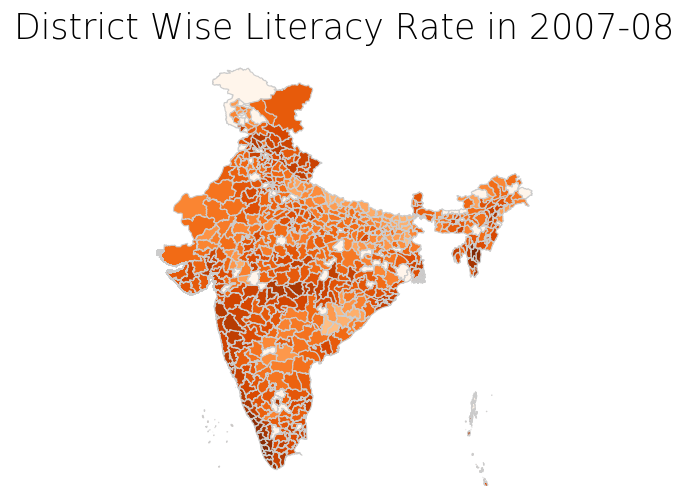
\includegraphics[width=0.9\textwidth]{Literacy_07_08.png}
    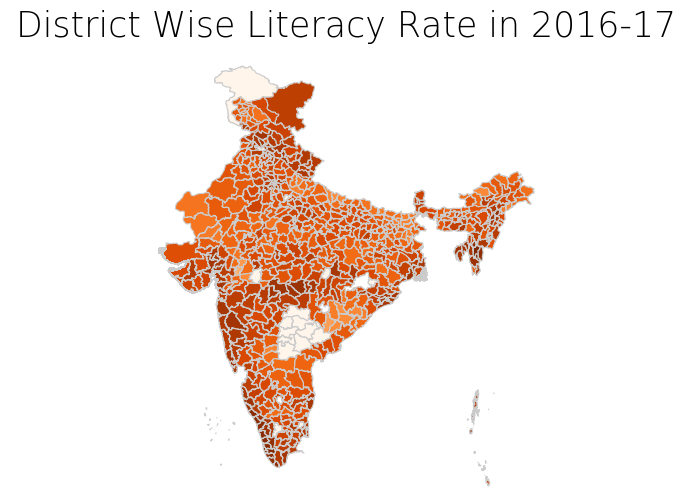
\includegraphics[width=0.9\textwidth]{Literacy_16_17.png}
    \caption{Figure showing distribution of literacy rate. Darker shades represent higher literacy rate}
    \label{fig:literacy_heatmap}
\end{figure}

\begin{figure}[h]
    \centering
    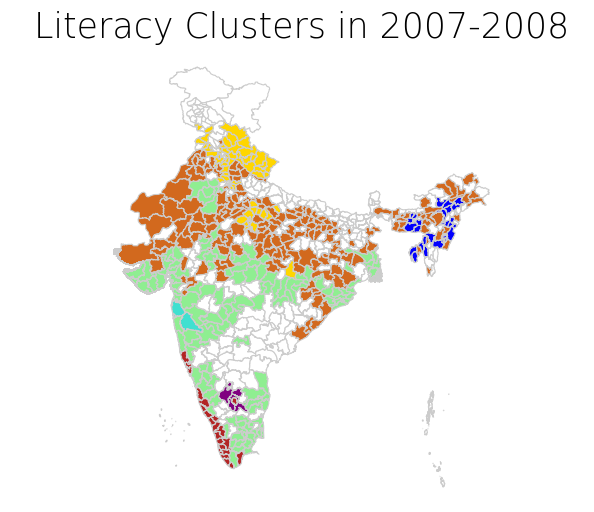
\includegraphics[width=0.8\textwidth]{Literacy_Clusters_07_08.png}
     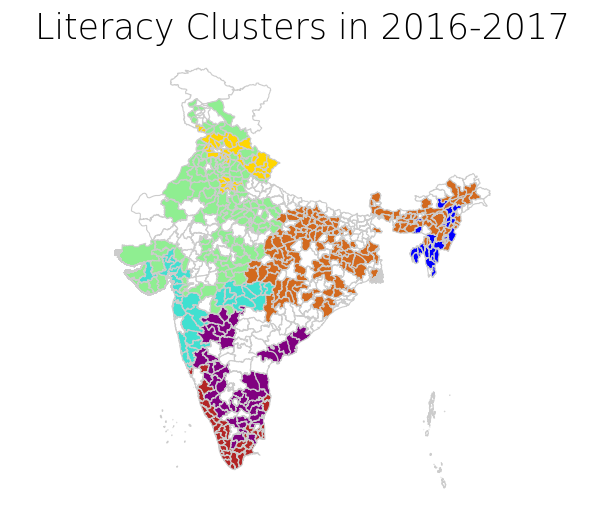
\includegraphics[width=0.8\textwidth]{Literacy_Cluster_16_17.png}
    \caption{Figure showing various literacy clusters. Different clusters are shown in different colors}
    \label{fig:literacy_clusters}
\end{figure}
\begin{figure}[h]
    \centering
    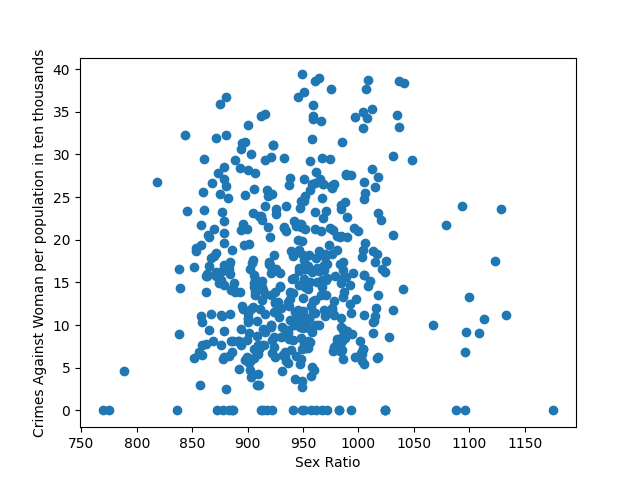
\includegraphics[width=0.8\textwidth]{sex_ratio_crimes_against_women_2016.png}
     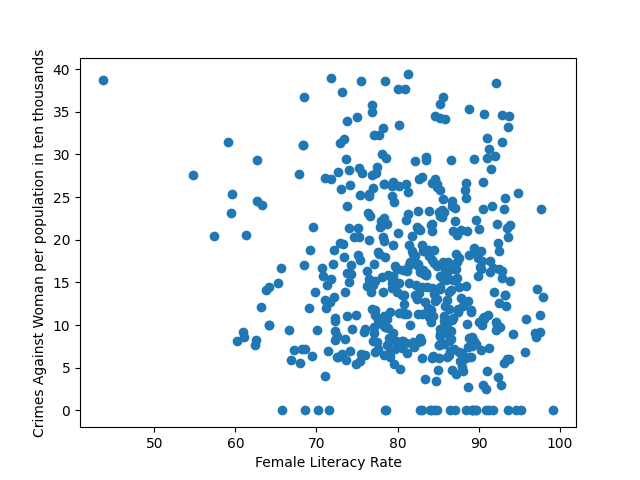
\includegraphics[width=0.8\textwidth]{female_literacy_rate_crimes_against_women_2016.png}
     \caption{Correlation between crime against women and educational parameters for 2016.}
    \label{fig:crime_scatter}
\end{figure}
\begin{figure}[h]
    \centering
    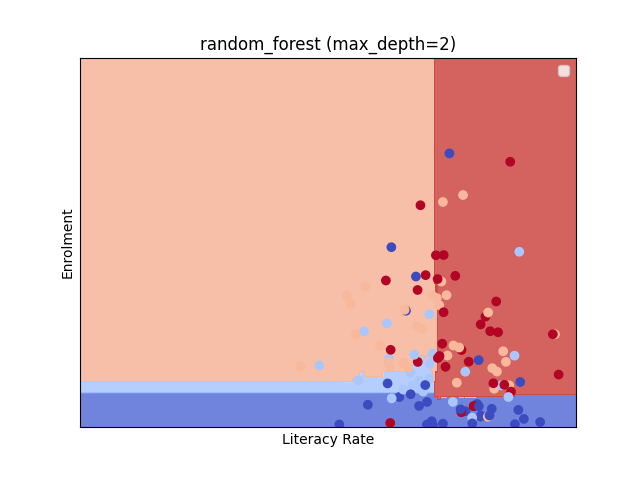
\includegraphics[width=0.45\textwidth]{random_forest(depth_limit=2)_literacy&incentive_vs_crime_2016.png}
     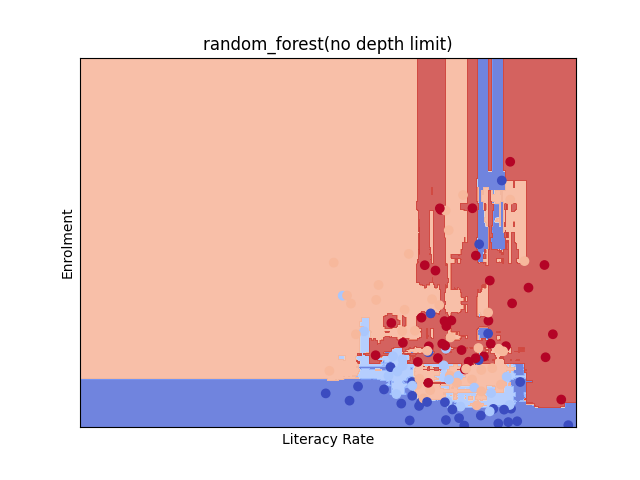
\includegraphics[width=0.45\textwidth]{random_forest(no_limit)_literacy&incentive_vs_crime_2016.png}
     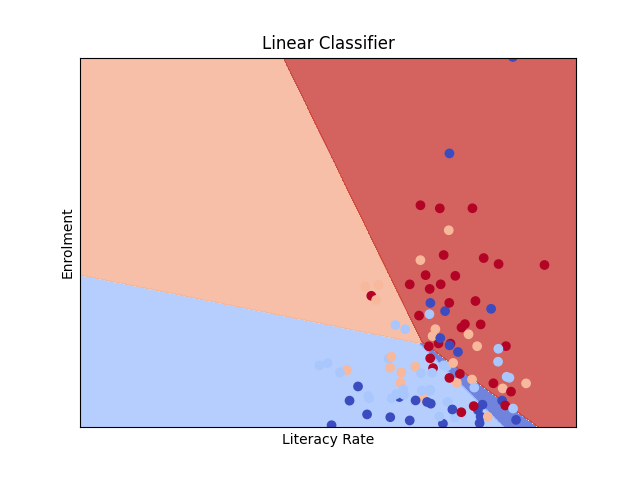
\includegraphics[width=0.45\textwidth]{linear_classifier_literacy&incentive_vs_crime_2016.png}
     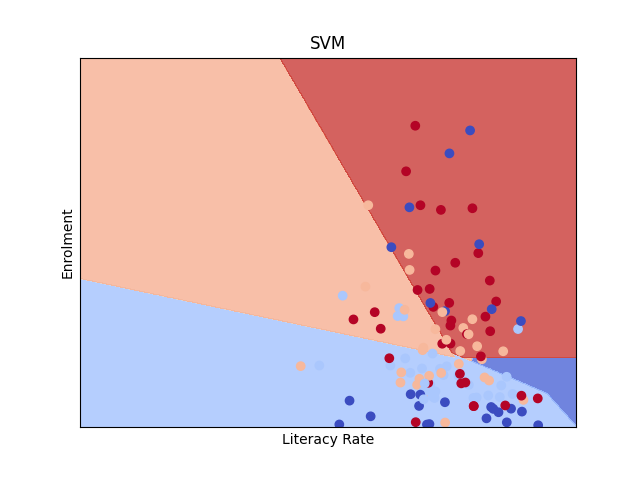
\includegraphics[width=0.45\textwidth]{svm_classifier_literacy&incentive_vs_crime_2016.png}
     \caption{Decision boundary for various models for predicting crime}
    \label{fig:crime_decision}
\end{figure}

\subsection*{Analyzing Total Enrollment vs Incentives}
In order to promote enrollment of students in schools, government provides incentives like free uniforms, free textbooks, attendance incentives and so on. We want to see how student enrollment in schools vary with the amount of incentives provided by the government. Our data-set consisted of the number of free uniforms and textbooks provided by the government. We also had the data for the number of student enrolled in government and private schools. To determine whether the incentives provided and the enrollment in schools have any correlation, we divided the districts into four type (low, mid low, mid high and high student enrollment) and trained a classifier which takes the incentives provided by the government as input and predicts the enrollment class. We did this twice, once considering the total number of students enrolled in government and private schools and once considering the total number of students enrolled in government schools only.\\

We trained a support vector classifier on our data with Gaussian kernel. The accuracy of the classifier when predicting enrollment classes vary from 65\% to 72\%. However, predicting enrollment in government schools based on the two parameters result in better accuracy of around 80\%. Figure \ref{fig:decision_boundary_enrollment} shows the decision boundary of our classifiers. We note few important points. First, predicting total number of students enrolled in government and private schools has lower accuracy. This may be because free incentives are usually distributed in government schools. Thus, private schools enrollment tend to be independent of incentives and hence add noise to the target. Predicting only enrollment in government schools give better accuracy. Secondly, data shows that number of uniforms distributed and number of textbooks distributed are in general proportional. However, there are certain districts in which large number of textbooks are distributed but not uniforms. Thirdly, we see that points in the lower left part of the curve i.e. areas where less incentives are provided are blue (representing lower enrollment) whereas data on the upper right i.e. areas with high number of incentives have enrollment. This point out to the fact that higher incentives motivate higher enrollment in schools.

\begin{figure}[h]
    \centering
    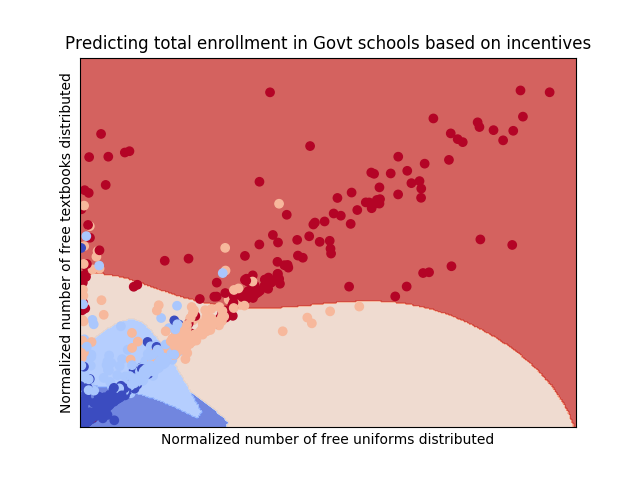
\includegraphics[width=0.8\textwidth]{Incentives-vs-govt-enrollment.png}
     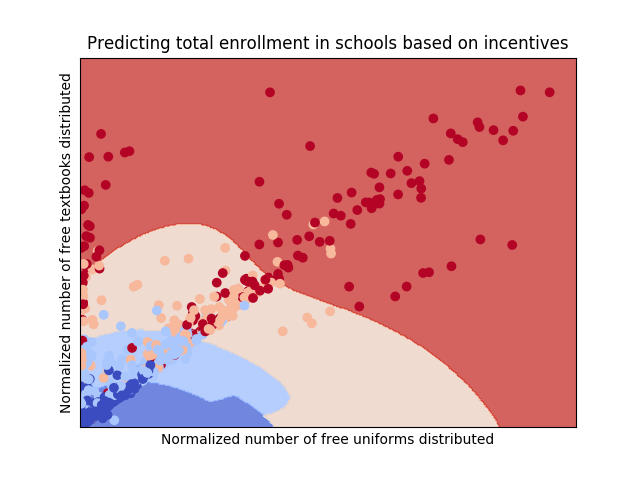
\includegraphics[width=0.8\textwidth]{Incentives-vs-total-enrollment.png}
    \caption{Decision boundary for classifiers predicting enrollment in schools from incentives distributed. Enrollment increase when going from dark blue to red.}
    \label{fig:decision_boundary_enrollment}
\end{figure}

\subsection*{Predicting Literacy Rate from Education parameters}
Another interesting thing to find will be whether or not the educational infrastructure and facilities available have an impact on the literacy rate of a district. To this end, we consider the following parameters: total number of government and private schools, total number of students enrolled in schools, incentives for education and enrollment of students in rural areas and try to predict the literacy rate of the district. We formulate this as a regression problem and train a support vector regression model.\\

To measure the performance of our classifier, we count the number of points for which the difference between the prediction of our model and the actual literacy rate is less than a certain threshold. Even with a threshold as high as 10\%, we find that the accuracy of our classifier is quite low, ranging from 50\% to 65\%. The low accuracy of our classifier can be attributed to several reasons. First, we have limited number of features available. Second, improvements in educational infrastructure and other parameters often take a long time to reflect as improved literacy rate. Thus, the classifier is expected to have lower accuracy.

\subsection*{Improvements in Educational Infrastructure over time}
Figure \ref{fig:education_time} shows how total number of schools, enrollment in schools etc. has changed over time. Several interesting points emerge from the data.
\begin{itemize}
    \item Between 2016 and 2007, there has been an increase in total number of government school with 90,000 new schools opening. This represents a 9.5\% increase in the number of government schools. We also see number 96000 new private schools which is equivalent to 40\% increase in private schools.
    \item There has been drop in enrollment in government schools. The number of students enrolled in private schools has increased by 3.9 crores whereas the number of students enrolled in government schools has decreased by 2.1 crores. Total number of students enrolled in private schools has almost doubled. Thus, we see a shift in favour towards private schools.
    \item Around 80\% of students in 2007 were enrolled in government schools. In 2016 this number has fallen to 60\%.
    \item Around 1 lakh more teachers were employed in government schools in 2016 then in 2007. For private schools this number is significantly higher and stands at 6 lakhs.
\end{itemize}
\begin{figure}[h]
    \centering
    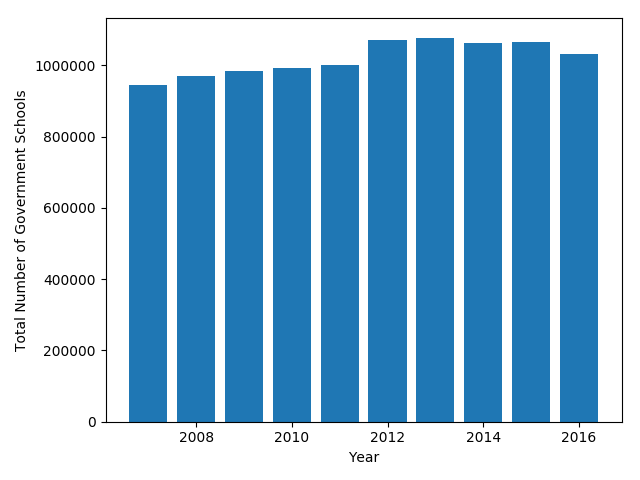
\includegraphics[width=0.45\textwidth]{GovtSchoolE.png}
    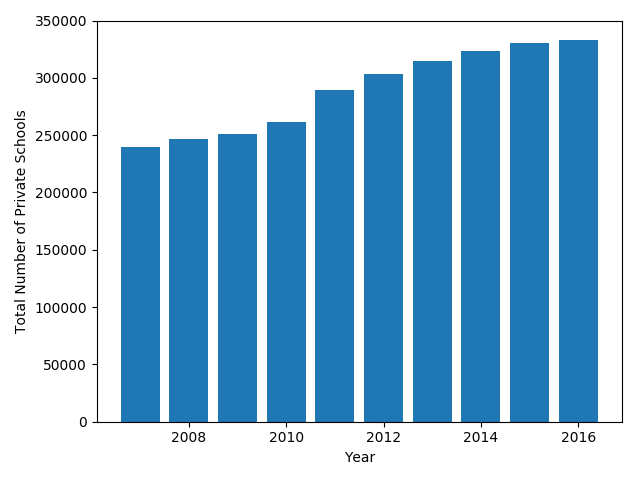
\includegraphics[width=0.45\textwidth]{PrvtSchoolE.png}
    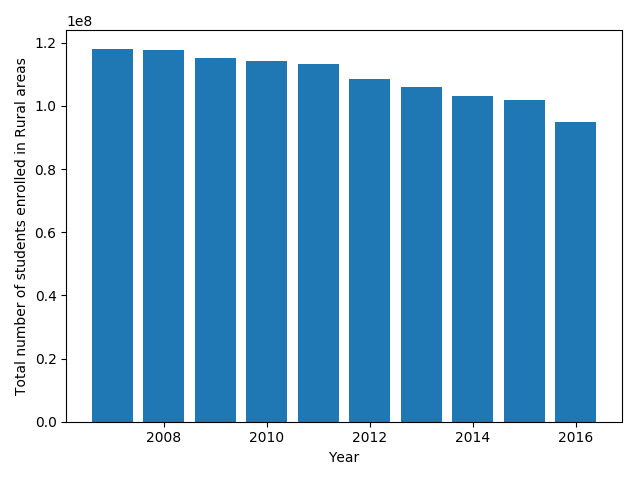
\includegraphics[width=0.45\textwidth]{RuralEnrolmentGovtE.png}
    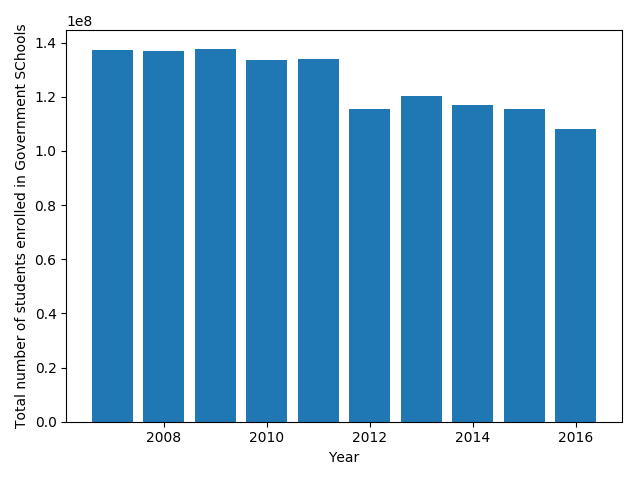
\includegraphics[width=0.45\textwidth]{TotalEnrolmentGovtE.png}
    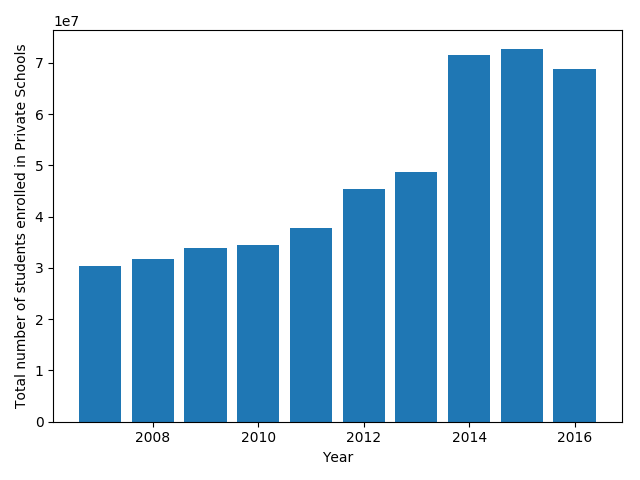
\includegraphics[width=0.45\textwidth]{TotalEnrolmentPrvtE.png}
    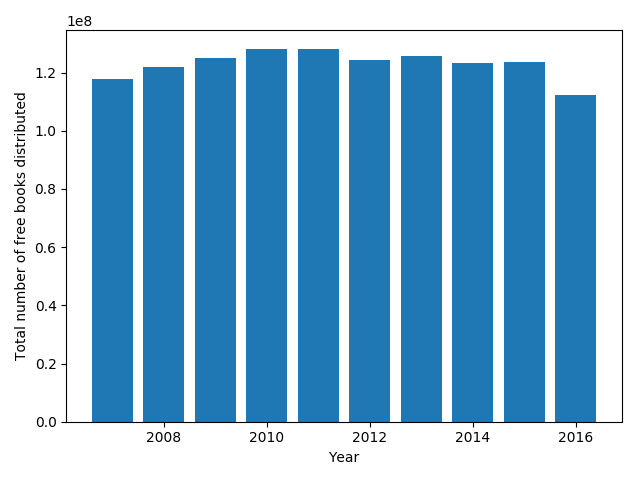
\includegraphics[width=0.45\textwidth]{TotalTextBookIncentives.png}
    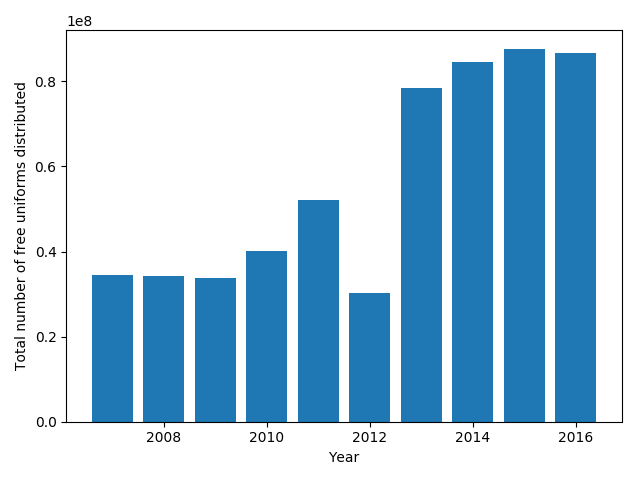
\includegraphics[width=0.45\textwidth]{TotalUniformIncentives.png}
    \caption{Figure showing change in various education parameters over time}
    \label{fig:education_time}
\end{figure}

\subsection*{Correlation between crime rate and educational parameters}
We explored various plausible correlations that might be existent between both of these.
We primarily relied on Pearson and Spearman coefficients and mutual information for checking the relations among these.\\
These metrics surprisingly indicated a very weak positive correlation between these parameters.\\
We repeated the analysis from 2013 to 2016 for all of these, since data was available for these years only for both crime and education.
The results obtained are concluded in Tables \ref{tab:pearson_coefficient} and \ref{tab:spearman_coefficient}.
\begin{table}[h!]
\centering
\begin{tabular}{||c c c c||} 
 \hline
 Parameter 1 & Parameter 2 & YEAR & Coefficient Value \\ [0.5ex] 
 \hline\hline
%  Pearson
 Total Schools & All Crimes & 2013 & 0.213 \\ 
 Total Schools & All Crimes & 2014 & 0.396 \\ 
 Total Schools & All Crimes & 2015 & 0.340 \\ 
 Total Schools & All Crimes & 2016 & 0.343 \\ 
 
 Literacy Rate & All Crimes & 2013 & -0.029 \\ 
 Literacy Rate & All Crimes & 2014 & 0.003 \\ 
 Literacy Rate & All Crimes & 2015 & -0.005 \\ 
 Literacy Rate & All Crimes & 2016 & -0.007 \\ 
    
 Sex Ratio & Crime Against Women & 2013 & -0.033 \\ 
 Sex Ratio & Crime Against Women & 2014 & -0.129 \\ 
 Sex Ratio & Crime Against Women & 2015 & -0.140 \\ 
 Sex Ratio & Crime Against Women & 2016 & -0.140 \\ 
 
 Total Schools & Crime Against Children & 2013 & 0.202 \\ 
 Total Schools & Crime Against Children & 2014 & 0.218 \\ 
 Total Schools & Crime Against Children & 2015 & 0.183 \\ 
 Total Schools & Crime Against Children & 2016 & 0.223 \\ [1ex] 
 \hline
\end{tabular}
\caption{Pearson coefficient for various parameters}
\label{tab:pearson_coefficient}
\end{table}
\begin{table}[h!]
\centering
\begin{tabular}{||c c c c||} 
 \hline
 Parameter 1 & Parameter 2 & YEAR & Coefficient Value \\ [0.5ex] 
 \hline\hline
%  Spearman
 Total Schools & All Crimes & 2013 & 0.064 \\ 
 Total Schools & All Crimes & 2014 & 0.508 \\ 
 Total Schools & All Crimes & 2015 & 0.486 \\ 
 Total Schools & All Crimes & 2016 & 0.511 \\ 
 
 Literacy Rate & All Crimes & 2013 & 0.044 \\ 
 Literacy Rate & All Crimes & 2014 & -0.003 \\ 
 Literacy Rate & All Crimes & 2015 & -0.017 \\ 
 Literacy Rate & All Crimes & 2016 & -0.038 \\ 
 
 Sex Ratio & Crime Against Women & 2013 & -0.005 \\ 
 Sex Ratio & Crime Against Women & 2014 & 0.031 \\ 
 Sex Ratio & Crime Against Women & 2015 & 0.045 \\ 
 Sex Ratio & Crime Against Women & 2016 & 0.052 \\ 
 
 Total Schools & Crime Against Children & 2013 & 0.083 \\ 
 Total Schools & Crime Against Children & 2014 & 0.124 \\ 
 Total Schools & Crime Against Children & 2015 & 0.177 \\ 
 Total Schools & Crime Against Children & 2016 & 0.209 \\
 
 Female literacy Rate & Crime Against Women & 2013 & -0.063 \\ 
 Female literacy Rate & Crime Against Women & 2014 & -0.042 \\ 
 Female literacy Rate & Crime Against Women & 2015 & -0.022 \\ 
 Female literacy Rate & Crime Against Women & 2016 & -0.048 \\
 School with computer & Cyber Crime & 2016 & -0.301 \\
 Total Schools & Crime by Juveniles & 2016 & -0.144 \\ [1ex] 
 \hline
\end{tabular}
\caption{Spearman coefficient for various parameters}
\label{tab:spearman_coefficient}
\end{table}

%  Spearman
Some important observations from the table is that as the sex ratios in the schools is improving, crime against women is decreasing across the districts as the correlation is negative, though it is not very strong. Also, there is a weak negative correlation between schools with computers and cyber crime, as expected. Also from table \ref{tab:spearman_coefficient}, we see there is a weak negative correlation between total schools and crime by juvenile and also against them, which was expected. Although some contrasting trends have also been observed, like Total Schools and all crime and crime against children show positive correlation. From table \ref{tab:spearman_coefficient}, we can see that female literacy rate is negatively correlated to crimes against women. The only problem here is that we did not find a statistically significant correlation between crime and education for any crime or education metric. This is quite counter-intuitive. Another counter-intuitive observation is a significant increase in crimes against children and all crimes with total number of schools, we can observe this in table \ref{tab:pearson_coefficient} and also table \ref{tab:spearman_coefficient}. There is no reasonable explanation that could account for this.\\

\subsection*{Analyzing Crime Rates based on education parameters of an area}
We wanted to create a machine learning model which could predict the reported crime of the area given its literacy rate and available educational infrastructure. We analysed the crime data and found that it was quite sparse for the year 2013 which was because of missing data and hence any model did not work well with 2013 and maximum accuracy we could get was around 25\%. However, we tried many different methods for other years. When we used a decision tree, an extremely over-fitting model was generated which gave full accuracy on the training set but negligible accuracy on the test set when we used held-out validation. This can be attributed to the small amount of data points.

As a standard corrective measure to improve the performance of decision tree, we used a random forest classifier. This improved accuracy to about 60\% which was further improved to 70\% when pruning was used. This was good but we thought of trying a different method, a support vector machine. It gave a decent accuracy with the small amount of data points used which was 75\%.  

Further, we modified the predicting crimes problem into a problem to predict the intensity of the crime rates.So for each year we classified the zones(districts) into 4 parts,i.e having very low crime rate, low-medium crime rate , high-medium crime rate and high rate.So we turned a regression problem into a classification problem, predicting the relative crime scenario of a district.
For creating this division, we used the training data-set among lowest (1/4)th crime into low crime, next (1/4) in low-medium and so on.
We selected total enrolment(government + private) of schools and the literacy rate as the parameters for predicting the total crime occurring in any district.
We normalised the total crime with the total population of an area, to account for uneven distribution of population with districts.Also the total enrolment was normalised, so as to avoid overflow issues for better results.


% Random Forest(max_depth=2)
% 2013
% 123 121 130 122
% 131 365 26.411290322580644
% 2014
% 127 126 127 127
% 342 165 67.45562130177515
% 2015
% 119 132 125 137
% 299 214 58.28460038986355
% 2016
% 133 116 125 133
% 332 175 65.48323471400394

% Random Forest
% 2013
% 124 118 118 122
% 139 343 28.83817427385892
% 2014
% 130 133 132 124
% 368 151 70.90558766859345
% 2015
% 119 126 125 131
% 343 158 68.46307385229541
% 2016
% 125 122 128 118
% 360 133 73.02231237322515

% SVM
% 2013
% 127 130 125 136
% 125 393 24.131274131274132
% 2014
% 128 133 132 123
% 380 136 73.64341085271317
% 2015
% 120 132 112 124
% 354 134 72.54098360655738
% 2016
% 125 139 140 120
% 395 129 75.38167938931298

% Linear Regressor
% 2013
% 127 133 127 128
% 126 389 24.466019417475728
% 2014
% 128 126 130 122
% 339 167 66.99604743083005
% 2015
% 130 133 119 131
% 370 143 72.12475633528265
% 2016
% 125 128 132 127
% 393 119 76.7578125

%  sex ratio in schools vs crime in pearson ka explanation, female literacy rate vs crime against women
% computer vs cyber crime spearman
% total school vs crime by  juvenile
% total school vs crime against children
\section*{Future Work}
The project explores how educational infrastructure and literacy rates are correlated and explores the improvements in educational infrastructure and Literacy rate over time. We find that certain parameters like enrollment of students and incentives are correlated but were not able to find a good model for predicting literacy rate from other educational parameters. This was partly due to limitations in available data. An interesting future work would be to procure better quality of data. This, however, is quite challenging task and requires significant time, field work and resources and can be done only by the government. Another future direction could be to try more powerful models like deep neural networks which can learn highly non-linear models.\\

During our analysis we tried to model crime as a function of education level. However, education and literacy rate are usually not the only parameter that determine crime rates. Factors like economic growth, strictness of law enforcement etc. also play an important role in determining crime rate. A more comprehensive analysis which takes into account all these factors is expected to achieve better results.\\

Models that determine parameters like crime rate, economic growth etc. can be used to determine optimal allocation of available resources. For instance, a model that models crime rate or economic growth on the basis of educational infrastructure can be used to allocate available resources like funds for providing incentives to students, new schools etc. such that the allocation results in speediest reduction in crime rates or accelerated economic growth.

\vspace*{-0.6cm}
\section*{Conclusion}
\vspace*{-0.4cm}
We proposed a strong negative correlation between the crime rate and the education parameters like literacy rate. But from the analysis, our proposition was not very well supported with the data provided. Though at places, we found weak correlations in support of our hypothesis, but we do not find it convincing enough to conclude our initial hypothesis. We could however get a reasonable accuracy for a model trained on the data.

In other areas of our analysis, like analyzing the variation of total enrollment in schools with incentives provided, we got a significant positive correlation especially in government schools indicating that incentives can be provided to promote education. Also the significance of private schools in education has increased over the years. This can be attributed to better quality education provided in these institutions. 

We also saw a general trend in the increase in literacy rate with increase in the number of schools across clusters. Many clusters got upgraded from 2007-08 to 2016-17. There is however very high variance in educational infrastructure and hence literacy rate across the country.
\vspace{-0.5cm}

\section*{References}
\vspace{-0.5cm}
\beginrefs
\bibentry{EDS} Education Data Source
{\it UDISE} :- \it{http://udise.in/drc.htm}
\bibentry{CDS} Crime Data Source  {\it NCRB} :-\it{https://ncrb.gov.in/en/crime-in-india-table-contents}
\bibentry{CODE} Link to Code  {\it Github} :-\it{https://github.com/adimishra1/DataMiningProject}
\bibentry{DATA} Link to Final Data  {\it Drive} :-\\\it{https://drive.google.com/drive/folders/1waYNAyPxsRpmmFtk\textunderscore SAuuWfWt8xTJI50?usp=sharing}




\endrefs

\end{document}



